\section{Deep learning}
%Review by \cite{LeCun2015DeepLearning}.\\

Before deep learning, raw data had to be transformed into an internal representation using manually crafted features usable for learners. In deep learning, these features are learned by itself, as it is a representation-learning method. Furthermore, different levels of representation can be used. Each level builds upon the previous one, starting from the input itself, and represents it in a more abstract way. These abstractions are generated as to recognize aspects of the input that are important for the task. Because of this, it is possible that small variations in the input have no influence on the abstraction and output.
As these abstractions are learned automatically, there is no need anymore to create internal representations manually, which require more work as it is different for every kind of task. The generated abstractions may also recognize useful patterns in the data that might not be represented using the hand-crafted features.\\

In supervised learning, our data set contains pairs of an input and the associated correct output, also called training examples. The goal is to be able to predict the correct output given the input. When doing classification, the output only has a finite set of possible values. As such, the classification algorithm can output a score for each possible output which signifies its certainty or confidence for that output being the correct one given the input. Because of this, we want the correct output to have the highest score.
In order to evaluate and improve the algorithm, we compute the error by calculating the differences between the computed output and the correct output. Using this error, the algorithm can then improve its predictions and subsequently reduce the error by adjusting its internal parameters. These parameters, also called weights, influence which output is generated given the input.\\

In order to adjust the weight vector, i.e. the internal parameters, a gradient is computed. This gradient indicates how the error would change when adjusting each parameter by an infinitely small amount, calculated using derivatives. The weight vector is then adjusted in the opposite direction of the gradient vector as to decrease the error. This is only possible if the values of the weight vector are continuous and they are differentiable w.r.t. the error.
%\todo{Something about local minima and that it's not a problem for deep neural networks}
This process continues until the error can't be reduced further, i.e. when it is in a local and/or global optimum.
It is possible to calculate this output, error and gradient for every training example and then adjusting the weights using the average of them.
In practice, however, stochastic gradient descent is used in order to reduce the computational cost and to have less chance of being trapped in local optima \citep{ML}.
Here, one calculates the errors, outputs and average gradient for only a few examples. This is again executed until the error does not decrease anymore. It is stochastic because only a few training examples are used, which results in an average gradient that can be noisy. However this is computationally less expensive than using all the training examples at every iteration.\\
After training, one can evaluate the trained algorithm on a different kind of data set, called a test set. This contains data that the algorithm has not trained on before. It is a way of seeing how well the algorithm has generalized beyond the given training examples.\\

One of the simplest classifier is one usable for 2 classes and which computes the linear combination of the input and a weight vector. The result is one number of which a threshold can be used to determine to which class the output belongs.
This algorithm however can only separate the input in simple regions, namely half-spaces separated by a hyperplane. This lack of granularity and influence of variance in input that is irrelevant for the classification task (e.g. shifted objects in a picture should still be classified correctly) is not suitable for complex tasks like image recognition, unless an adequate feature extractor is applied first. Generic methods like kernel methods can be applied but are not guaranteed to work well for the task.
Generally, feature extractors need to be developed manually in order to represent the aspects of the input that are important. This, however, requires more work and requires knowledge about the domain and the task.

In deep learning, the important aspects of the input can be detected automatically by combining different modules in order to get higher abstractions and to eventually generate output.
Most of these modules contain weights which can be trained.

\todo{Remove or rewrite this}
As already explained, stochastic gradient descent is used in order to reduce the error. This method requires however gradients to be computed. To do this, we use backpropagation. This requires that there exists a derivative of each computation. First, these are applied to the weights producing the final output (using the directly received error), and then by working backwards and propagating the gradient (using the chain rule) to the weights that directly handle the input.

In most of the applications using deep learning, feedforward neural networks are used. Here the input and output have a fixed size and the input is processed, possible using multiple layers, in order to produce the output.
The linear combination computed to go from one layer to the next can also pass through a non-linear function. One of the most popular is the rectified linear unit (\textit{ReLU}). This uses the formula $f(z) = max(0,z)$. Other possibilities include the \textit{tanh} function ($f(z) = tanh(z)$) and the sigmoid function ($f(z) = \frac{1}{1 + e^{-z}}$). \textit{ReLU} is the most popular for deep learning however as it learns much faster when having a lot of layers.

Layers that are between the input and output units are called hidden layers. These process the input in a non-linear way such that the categories become linearly separable. These hidden layers can be thought of as feature extractors.

Local minima might seem like a problem for neural networks, but in practice they are rarely a problem, according to theoretical and empirical results \citep{choromanska2015loss}.
Instead, there are more saddle points. Here, the gradient is zero and the surface curves up in most of the dimensions and curves down in the others. Generally a lot of such points are present, but they all have the same value for the objective function (the error).\\

\subsection{Convolutional neural networks}
Convolutional neural networks are neural networks that are inspired by the way the visual cortex of an animal works. These networks get as input data in multi-dimensional arrays, such as 2-dimensional images with pixel intensities as the third dimension for example.\\
A convolutional neural network is structured as a series of stages, which are combinations of layers. In the first stages, convolutional layers and pooling layers are used.
In a convolutional layer, units are organized in feature maps. Each of these units is connected to a patch in the feature maps of the previous layer through a matrix of weights that is called the filter bank. The filter bank matrix then slides over the feature map, does an element-wise computation of the 2 matrices and sums the results. The filter bank is then moved by a certain amount, called the stride. All units in a specific feature map of a layer use the same filter bank.
This is done because local groups of values may be correlated and as such may have the same weights. This reduces the amount of weights that need to be trained. Furthermore, certain concepts and local statistics (of images) may be invariant to the location. A certain pattern or motif in an image might appear in different places of the image but may have the same meaning.\\
The result of this convolutional operation (which is linear) operation is again a feature map and can then be passed to a non-linear function such as a \textit{ReLU}.\\

These convolutional layers are then combined with pooling layers. Instead of detecting local conjunctions of features from the previous layer, pooling tries to merge semantically similar features into one. This is necessary because the positions of features that form a motif are not exact and can vary somewhat. It may not matter for example that an object is close or far in an image.
To detect the motifs more reliably, we course-grain their features. The typical pooling units compute the maximum or average of a local patch of units in one or a few feature maps. The neighboring pooling units do the same for patches that are shifted by one or more rows and/or columns and as such creating an invariance to small shifts and distortions.\\
A typical layout of a convolutional neural network is shown in Figure~\ref{fig:cnnlayout}, while a hierarchy of features extracted using a convolutional neural network is shown in Figure~\ref{fig:cnnfeatures}.\\
\begin{figure}[htb]
    \centering
    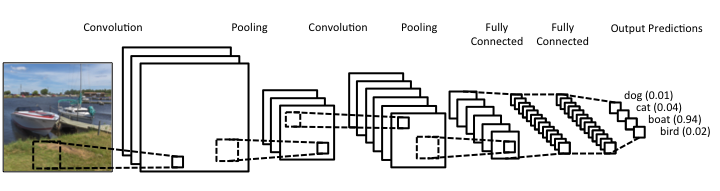
\includegraphics[width=\linewidth]{images/cnnlayout.png}
    \caption[Convolutional neural network layout]{Layout of a typical convolutional neural network, which uses convolutional layers, pooling layers and fully connected layers in order to detect an object in an image. Source: \url{https://www.clarifai.com/technology}}
    \label{fig:cnnlayout}
\end{figure}
\begin{figure}[htb]
    \centering
    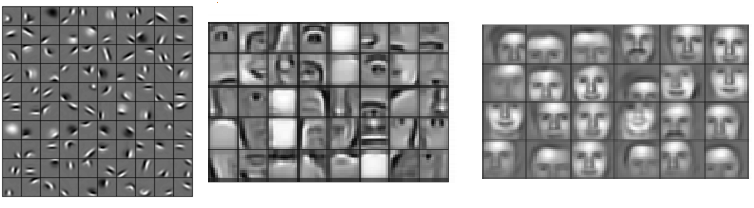
\includegraphics[width=\linewidth]{images/cnnfeatures.png}
    \caption[Convolutional neural network features hierarchy]{A hierarchy of features with as low-level features contours of faces. A more complex layer represents parts of faces. The final layer shows whole faces and can be used for classification or regression. Note that these features don't always have an intuitive meaning. Source: \cite{conf/icml/LeeGRN09}.}
    \label{fig:cnnfeatures}
\end{figure}

An example of a convolutional neural network is ConvNet, a convolutional network architecture that achieved many successes. Here, two or three of these convolutions, non-linearities and poolings are stacked. Afterwards, a convolutional layer and fully-connected layer follow.\\

\subsection{Recurrent Neural Networks}
Recurrent neural networks (RNNs) are used to process sequential data such as speech and language. Here, an input sequence is processed one element at a time. The first RNNs used a state vector in their units that contains history about the past elements in the sequence. This is visualized in Figure \ref{fig:rnnunrolled}.
\begin{figure}[htb]
\centering
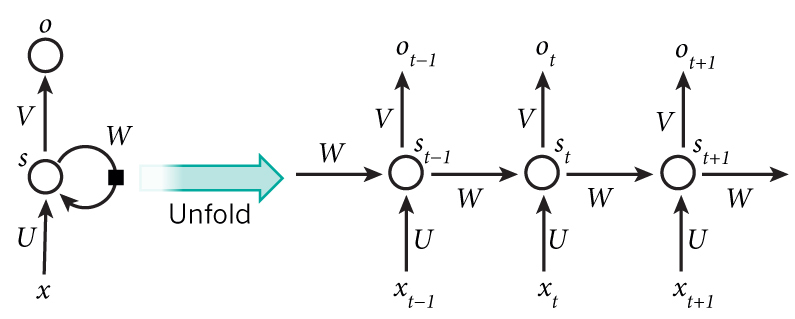
\includegraphics[width=0.8\linewidth]{images/RNN-unrolled.jpg} %source: http://www.wildml.com/2015/09/recurrent-neural-networks-tutorial-part-1-introduction-to-rnns/
\caption[Recurrent neural network]{A recurrent neural network in which each state (hidden unit) is passed to the next one. $x_t$ and $o_t$ are respectively the input and output at time step $t$. $s_t$ is the output of a hidden layer and depends on the input and the hidden unit at the previous time step: $s_t = U*x_t + W*s_{t-1}$. Note that the same weights $U$, $V$ and $W$ are used at each time step. Source: \cite{LeCun2015DeepLearning}.}
\label{fig:rnnunrolled}
\end{figure}
%The above diagram has outputs at each time step, but depending on the task this may not be necessary. For example, when predicting the sentiment of a sentence we may only care about the final output, not the sentiment after each word. Similarly, we may not need inputs at each time step. The main feature of an RNN is its hidden state, which captures some information about a sequence.

Training them was a problem because of the vanishing or exploding gradients, as these gradients either shrink or grow at every time step. Theoretical and empirical evidence has shown that it is hard for these kind of networks to store information long enough and that they have difficulties to learn the long-term dependencies \citep{bengio1994learning}.\\ %Sources for this: http://people.idsia.ch/~juergen/SeppHochreiter1991ThesisAdvisorSchmidhuber.pdf and http://www-dsi.ing.unifi.it/~paolo/ps/tnn-94-gradient.pdf

To learn RNNs, we also need to change the backpropagation algorithm in order to handle with the different time steps. Here, the error (for one training example) is just the sum of the errors at every time step: $e = \sum_t e_t$. The adapted backpropagation algorithm, called backpropagation through time (BPTT), also just sums up the gradient at every time step for every set of weights:  $\frac{\partial E}{\partial W} = \sum_t \frac{\partial E_t}{\partial W}$. For the weights $U$ and $V$ of Figure \ref{fig:rnnunrolled}, the gradients are computed just as in normal backpropagation. For $W$ however, we depend on the previous state, which cannot simple be treated as a constant, and must be replaced as well. Because of this, we get:
\begin{equation}
\frac{\partial E_t}{\partial W} = \sum_{k=0}^t \frac{\partial E_t}{\partial \hat{y}_t} \frac{\partial \hat{y}_t}{\partial s_t} \frac{\partial s_t}{\partial s_k} \frac{\partial s_k}{\partial W}
\end{equation}
We see that training can be hard when the sequences are long, because we need to propagate back through the first time step.\\

For the \textit{tanh} and \textit{sigmoid} function, the derivative is $0$ at both ends. This means that the gradients in other layers will also go towards zero and for small values in the matrix multiplications the gradient values are shrinking exponentially fast and become nearly zero after a few time steps. Because of this, steps far away won't contribute much to what you're currently computing, and as such the long-term dependencies are small. If the values of the partial derivatives are high however, we could get exploding gradients. These are however easier to detect and solve, because the value of the gradients will be too high to be presented by a variable in the programming language. The problem can also easily be solved by restricting the value in a certain range.\\ %source: http://www.jmlr.org/proceedings/papers/v28/pascanu13.pdf
The problem of vanishing gradients can be solved by a better initialization of the weights, by regularization and by another non-linear function, namely the already explained \textit{ReLU}.
For this function, the derivative is either 0 (when $z<0$) or 1 ($\frac{\partial z}{\partial z} = 1$).\\

A way of solving this is using a long short-term memory. This is a combination of different units and has an explicit memory. One of the units has a connection with itself and is used to accumulate or forget the stored information. It can be learned using another unit to know when to forget something and when to remember past information.\\
An LSTM architecture consists of different parts:
\begin{itemize}
\item An input gate $i$ that determines how much of the newly calculated state should be let through into the memory: $i = \sigma (x_tU^i + s_{t-1}W^i)$.
\item A forget gate $f$ that determines how much of the previous state you want to let through: $f = \sigma (x_tU^f + s_{t-1}W^f)$.
\item An output gate $o$ that determines how much of the internal hidden state you want to output to the next layer: $o = \sigma (x_tU^o + s_{t-1}W^o)$.
\item A candidate hidden state $g$ that is based on the input of the current time step and the state of the previous time step: $g = tanh(x_tU^g + s_{t-1}W^g)$.
\item An internal memory $c_t$ that is the sum of a fraction of the memory of the previous time step (determined by the forget gate) and a fraction of the candidate state (determined by the input gate): $c_t = c_{t-1} \circ f + g \circ i$.
\item Finally, the output hidden state $s_t$ is a fraction of the $tanh$ of the memory $c_t$, determined by the output gate: $s_t = tanh(c_t) \circ o$
\end{itemize}
Here, $U^i$ is for example one of the weight vectors for the input gate. The $\sigma$ function means the sigmoid function. $\circ$ refers to the dot product, i.e. $x \circ y = \sum_i^N x_i y_i$.\\
We can almost get the original RNN by setting the input and output gate weights to 1 and the forget gate weights to 0. The only difference is the $tanh$ function used to compute the output hidden state, which squashes the result more (along with the $tanh$ used to compute the candidate hidden state).\\
The architecture of an LSTM cell is shown in Figure~\ref{fig:lstm}.
\begin{figure}[htb]
    \centering
    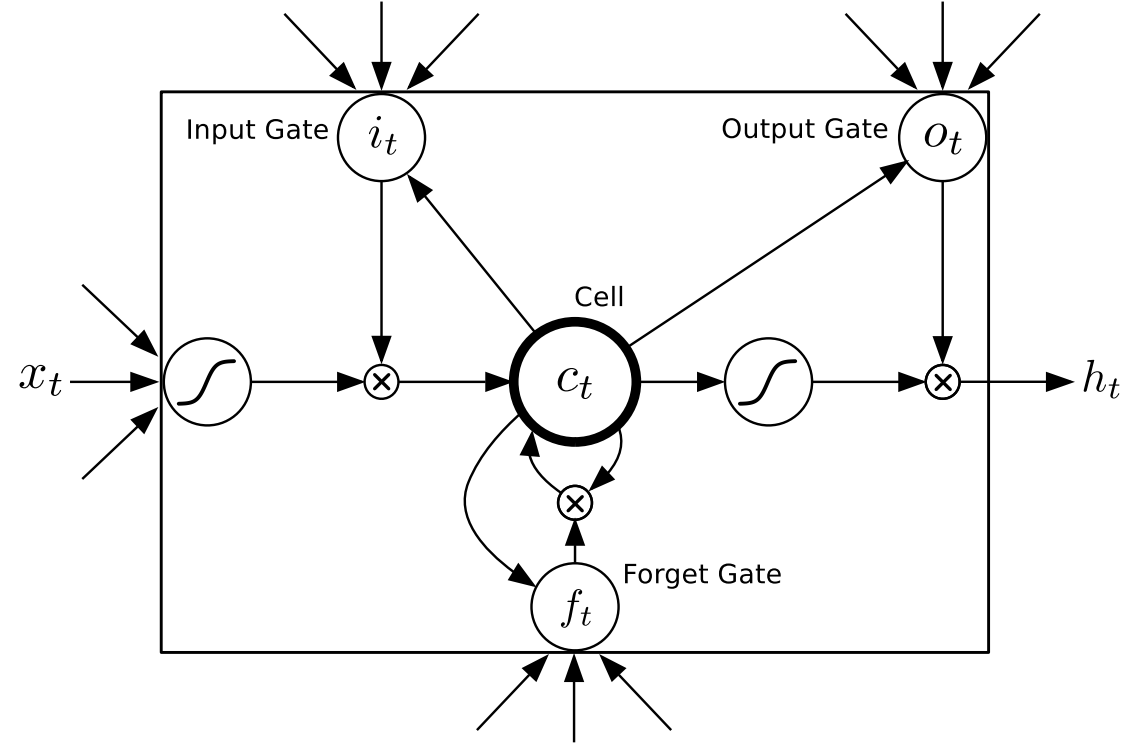
\includegraphics[width=\linewidth]{images/lstm.png}
    \caption[Long short-term memory cell]{The architecture of an LSTM cell. Source: \cite{journals/corr/Graves13}.}
    \label{fig:lstm}
\end{figure}
Another kind of recurrent unit is the Gated Recurrent Unit (GRU), which was introduced by \cite{Cho2014LearningTranslation}. It is simpler than LSTM but yields similar results. A GRU unit consists of the following parts:
\begin{itemize}
\item The update gate $z$ determines how much of the previous memory we want to keep, based on the input and the previous hidden state: $z = \sigma (x_tU^z + s_{t-1}W^z)$.
\item The reset gate $r$ says how much of the previous hidden state we want to combine with the current input, based on the previous hidden state and the input themselves: $z = \sigma (x_tU^r + s_{t-1}W^r)$.
\item Again a candidate hidden state $h$ that actually combines the previous hidden state and the input, using its own weights and the information from the reset gate: $h = tanh(x_tU^h + (s_{t-1} \circ r)W^h)$.
\item A new output hidden state based that combines all the previous information: $s_t = (1-z) \circ h + z \circ s_{t-1}$.
\end{itemize}
As we can see, the non-linearity function $tanh$ is only used once here. We also have no internal memory $c_t$ here. Instead, we use the update gate $z$ to combine the forget and input gate of the LSTM. The reset gate here is applied to the previous hidden state. As such, resetting in the LSTM architecture is done here using both the update gate and the reset gate. By always setting the reset gate to $1$ and the update gate to $0$ we get again the classic RNN architecture. The architecture of a GRU cell is visualized in Figure~\ref{fig:gru}.\\
\begin{figure}[htb]
    \centering
    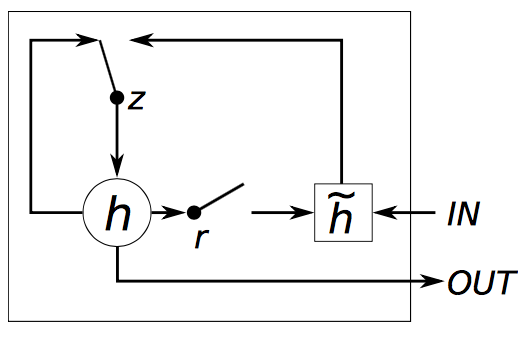
\includegraphics[width=0.6\linewidth]{images/gru.png}
    \caption[Gated Recurrent Unit cell]{Gated Recurrent Unit cell. Source: \cite{journals/corr/ChungGCB14}.}
    \label{fig:gru}
\end{figure}

Other networks with memory include a Neural Turing Machine, in which a tape-like memory is used from which the network can read or write.\\
Another kind is a memory network, in which a normal network is augmented by a associative memory.\\

\subsection{Dropout}
Dropout is a way to prevent overfitting. It does so by randomly leaving out some visible or hidden units. As a result, all incoming and outgoing connections to these temporarily removed units are also removed and the algorithm can't rely on these connections. The simplest way of determining if a unit has to be removed is by removing it with a certain probability $p$, e.g. $p=0.5$. This value can also be determined by validation. As each unit can be present or not when using the network, for $n$ units there are $2^n$ possible networks.
By learning each time using a possibly different network, we have a way of combining multiple models where each model is trained only a few times and most weights are shared between other models. Dropout is only used when training. In the testing phase, no units are removed. Here, however, we multiple the outgoing weights of each unit by there probability $p$.
This is done to make sure that the the \textit{expected} output for any hidden unit is the same as the actual output at test time.

In deep learning there are usually millions of these weights which can each be adjusted and can influence the output.
